\newpage
\section{Aplikacja mobilna - kontroler}

\begin{center}
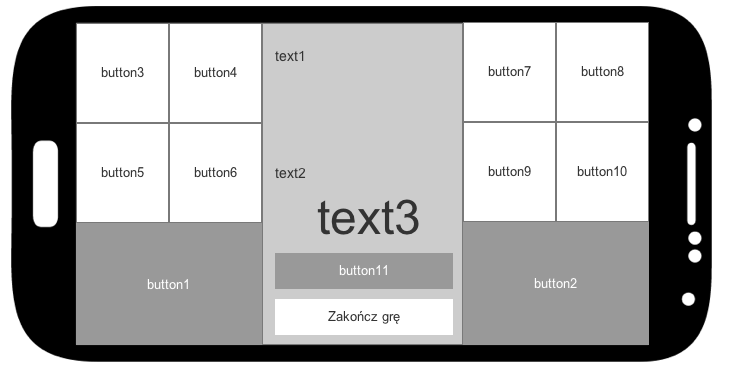
\includegraphics[width=1\textwidth]{images/button_mockup.png}
\captionof{figure}{
Makieta - układ przycisków
}
\end{center}
\paragraph{}
Głównym założeniem było stworzenie uniwersalnego kontrolera przygotowanego pod dowolny rodzaj gry, bądź innej wizualizacji stworzonej w środowisku Unity. Podczas uruchomienia kontrolera serwer wysyła statusy przycisków oraz pól tekstowych.


\begin{center}
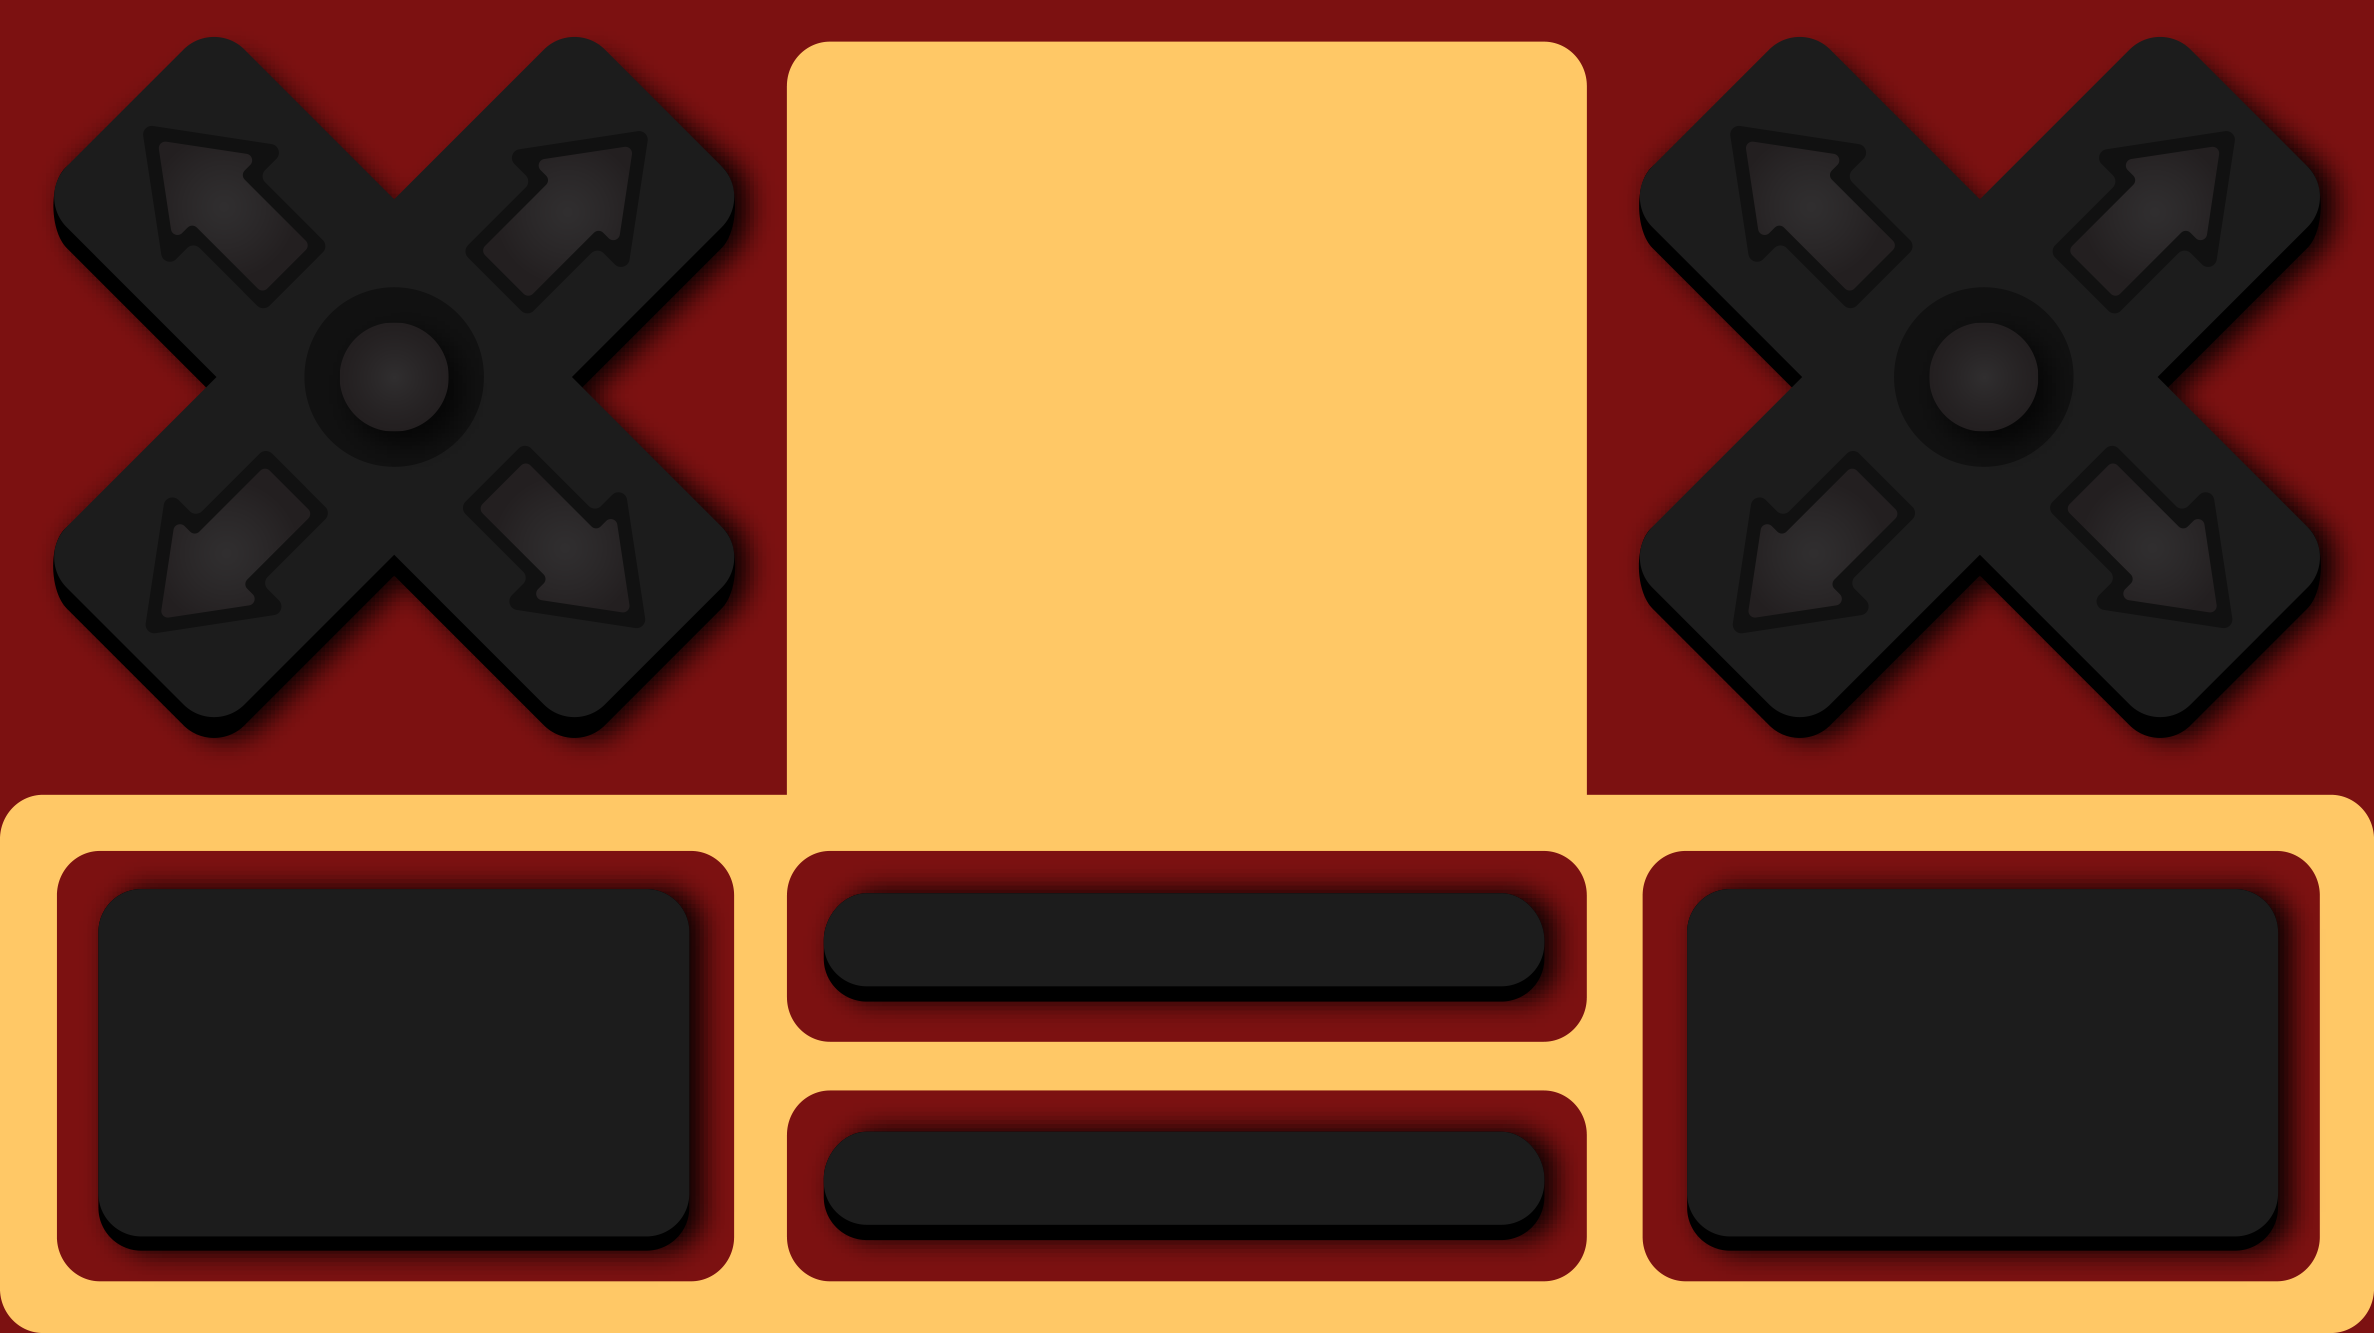
\includegraphics[width=1\textwidth]{images/graph1.png}

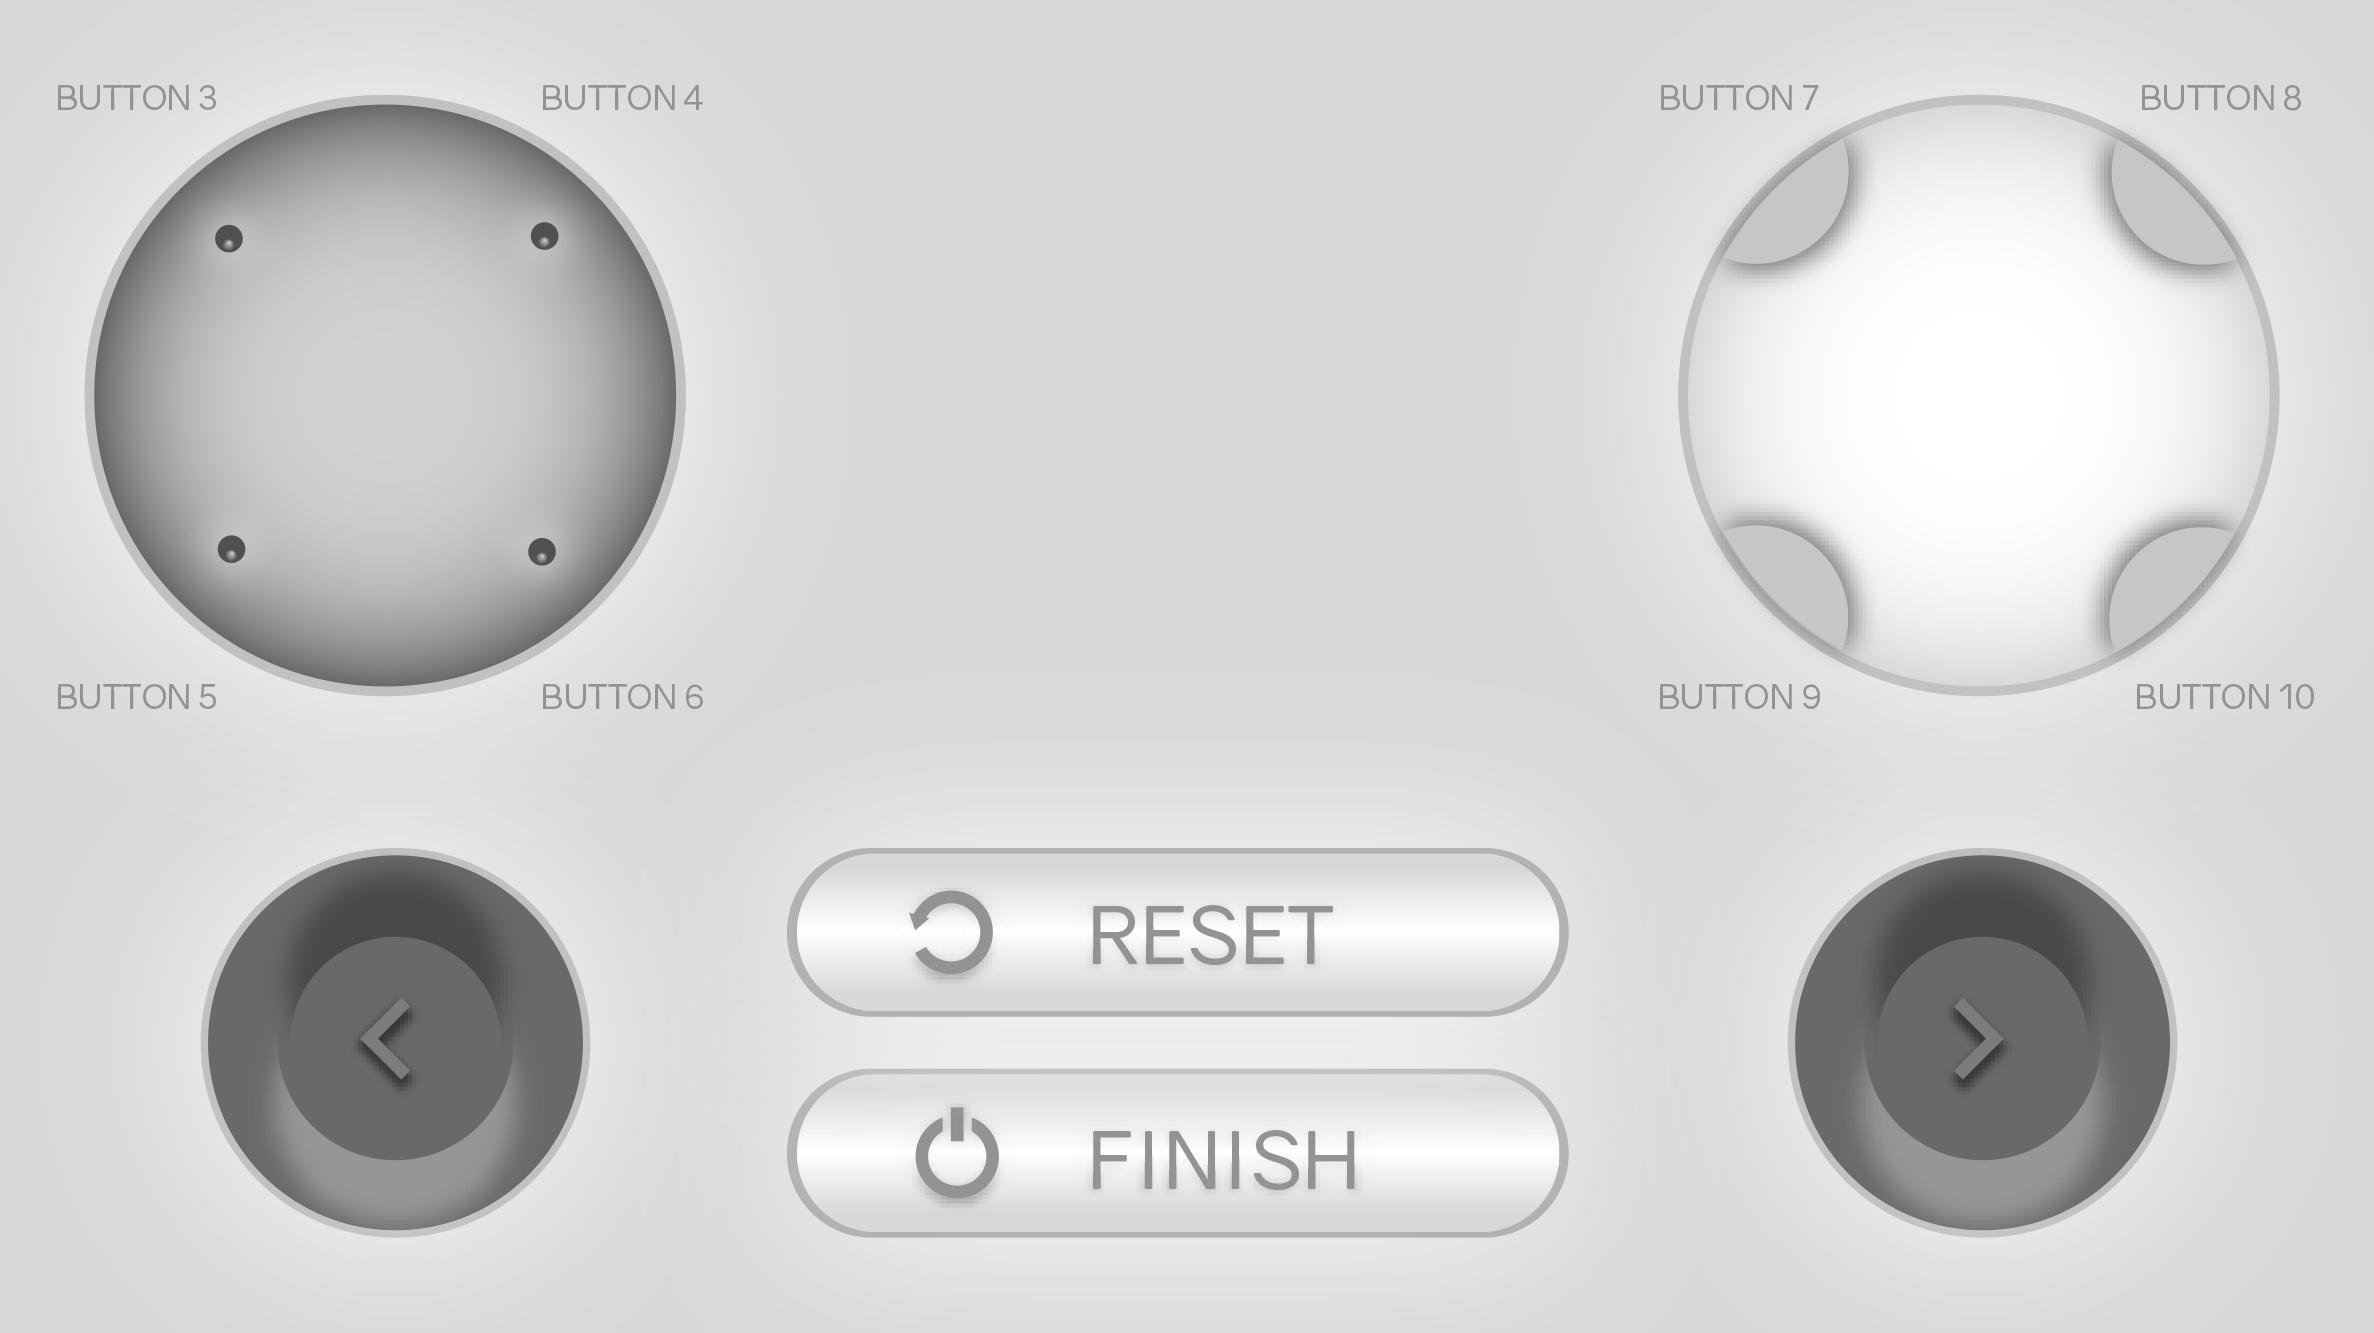
\includegraphics[width=1\textwidth]{images/graph2.png}
\captionof{figure}{
Przykładowa wizualizacja kontrolera
}
\end{center}

\subsection{Przyciski}
\paragraph{}
Każdy przycisk może zostać skonfigurowany poprez ustawienie tekstu. Dodatkowo można zablokować przycisk podczas gdy nie jest on potrzebny w danym czasie. 
Jednym z główny założeń architektonicznych był rozdzielenie warstwy widoku od logiki biznesowej. Ustalono, że stworzenie nowego przycisku odbywać się będzie wymagało tylko dodania definicji w warstwie widoku (plik layout w formacie XML).

\begin{lstlisting}[language=XML]
<pl.pjatk.remotecontroller.CustomButton
    app:name="button2"
    android:layout_gravity="center_horizontal"
    android:layout_height="wrap_content"
    android:layout_width="wrap_content"
/>
\end{lstlisting}
\captionof{lstlisting}{
	Przykład zdefiniowanego przycisku
}
\paragraph{}
Na potrzeby realizacji powyższego założenia stworzono klasę CustomButton, która jest rozszerzeniem (dziedziczy bezpośrednio) klasy Button znajdującej się w pakiecie  android.widget.
\paragraph{}
Każdy z przycisków musi posiadać własną nazwę kodową, gdyż serwer podczas komunikacji sieciowej identyfikuje przycisk poprzez unikalny klucz. Domyślnie w środowisku Android każdy komponent wizualny może posiadać swoje Id, jednakże jest one reprezentowane poprzez liczbę typu Integer.
Dla ułatwienia dalszego rozwoju aplikacji postanowiono stworzyć nowy atrybut. Ich definicje umieszczas ię w formacie XML w pliku attrs.xml

\begin{lstlisting}[language=XML]
<resources>
    <declare-styleable name="CustomButton">
        <attr name="name" format="string" />
    </declare-styleable>
</resources>
\end{lstlisting}
\captionof{lstlisting}{
    Definicja atrybutu o nazwie name
}

\paragraph{}
W konstuktorze poza domyślnymi wywołaniami klasy bazowej Button zapisywana jest wartość atrybutu name do zmiennej o tej nazwie oraz następuje wstępna konfiguracja przycisku.

\begin{lstlisting}[language=Java]
private static HashMap<String, CustomButton> buttons = new HashMap<String, CustomButton>();

private void setUp() {
    buttons.put(getName(), this);
    setText(getName());

    setOnClickListener(new View.OnClickListener(){
        @Override
        public void onClick(View v) {
            try {
                new Runner().execute(getName());
            } catch (Exception e) {
                Toast.makeText(getContext(), R.string.SendError, Toast.LENGTH_SHORT).show();
            }
        }
    });
}
\end{lstlisting}
\captionof{lstlisting}{
    Konfiguracja w klasie CustomButton
}
\paragraph{}
{\color{red}opisac co tu sie dzieje}


\subsection{Użycie styli}
\paragraph{}
Dodatkowym wymaganiem było umożliwienie szybkiej zmiany wyglądu przycisków.
\paragraph{}
Aby utrzymać porządek w kodzie kontrolera postaniowiono zastosować style do powtarzalnych elementów. W pliku styles.xml można zdefiniować własny styl - zbiór właściwości wizualnych mających posiadać np. wszystkie przyciski.


\begin{lstlisting}[language=XML]
 <style name="MyButton" parent="@android:style/Widget.Button">
    <item name="android:layout_width">wrap_content</item>
    <item name="android:layout_height">wrap_content</item>
    <item name="android:textColor">#fff</item>
    <item name="android:background">@color/colorPrimary</item>
    <item name="android:radius">0dp</item>
    <item name="android:typeface">monospace</item>
</style>

<style name="MyButtonDark" parent="MyButton">
    <item name="android:textColor">#f2f2f2</item>
    <item name="android:background">#000</item>
</style>
\end{lstlisting}
\captionof{lstlisting}{
   Przykład styli dla przycisku
}

\begin{lstlisting}[language=XML]
<Button
    style="@style/MyButton"
    android:text="Button 2"
    android:id="@+id/button2"
    android:layout_gravity="center_horizontal"
    android:layout_width="match_parent"
    android:layout_height="match_parent" />
\end{lstlisting}
\captionof{lstlisting}{
   Użycie stylu wraz z nadpisaniem właściwości
}

\paragraph{}
Jednakże z poziomu kodu źródłowego nie ma możliwości zmiany styli w trakcie uruchomienia aplikacji.  Dlatego też zrezygnowano z pełnego opisu warstwy GUI w plikach XML. Przyciski (w odpowiednim już stylu) są generowane bezpośrednio w kodzie źródłówym aplikacji (pliki Java). 
\paragraph{}
{\color{red}opsiać jak to sie robi inaczej + przykład implementacji klasy własnego buttona}

\subsection{Informacje tekstowe}
\paragraph{}
Pola tekstowe mogą mieć ustawioną dowolną treść w dowolnym czasie.

\subsection{Komunikacja sieciowa}
\paragraph{}
{\color{red}tutaj opisać implementacje warstwy komunikacyjnej}
